% !TeX encoding = UTF-8

% =========================================================
% 西南财经大学本科生毕业论文（设计）LaTeX 模板主文档
% 依据：《西南财经大学本科生毕业论文（设计）撰写与印制规范》
% =========================================================

\documentclass[type=bachelor, openany, oneside]{sjtuthesis}
% 文档类选项：
%   type=bachelor        % 论文类型为学士/本科
%   oneside / twoside    % 单面或双面排版模式（规范要求正反双面打印，提交电子稿可选 oneside）
%   openany / openright  % 奇数页或任意页开始新章

% 载入全局配置与宏包
% !TEX root = ./main.tex

% =========================================================
% 西南财经大学本科生毕业论文（设计）宏包配置与全局格式
% 依据：《西南财经大学本科生毕业论文（设计）撰写与印制规范》
% =========================================================

% 使用发行版提供的文档类，拒绝旧接口版本。
\IfClassAtLeastTF{sjtuthesis}{2026/02/26}{}{%
  \PackageError{swufe}{SJTUTeX 2.3.1 or newer is required}%
    {Update the sjtutex package in your TeX distribution.\MessageBreak
     On Overleaf, select TeX Live 2026 or newer.}%
}

\ExplSyntaxOn

% ---------------------------------------------------------
% 1. 本科论文信息与开关（单套字段，不区分语言）
% ---------------------------------------------------------
\tl_new:N \l__swufe_info_grade_tl
\tl_new:N \l__swufe_info_final_date_tl
\tl_new:N \l__swufe_info_display_title_tl
\tl_new:N \l__swufe_info_title_second_tl
\bool_new:N \g__swufe_citation_superscript_bool
\bool_new:N \g__swufe_bibliography_bib_bool
\tl_new:N \l__swufe_bibliography_bib_file_tl
\tl_new:N \l__swufe_bibliography_tex_file_tl

\keys_define:nn { sjtu }
  {
    review              .bool_gset:N = \g__sjtu_review_bool ,
    citation-superscript .bool_gset:N = \g__swufe_citation_superscript_bool ,
    bibliography .meta:nn = { sjtu / bibliography } {#1} ,
  }
\keys_define:nn { sjtu / bibliography }
  {
    source .choice: ,
    source / bib .code:n = { \bool_gset_true:N \g__swufe_bibliography_bib_bool } ,
    source / tex .code:n = { \bool_gset_false:N \g__swufe_bibliography_bib_bool } ,
    bib-file .tl_set:N = \l__swufe_bibliography_bib_file_tl ,
    tex-file .tl_set:N = \l__swufe_bibliography_tex_file_tl ,
  }
\keys_define:nn { sjtu / info }
  {
    % 修改完整标题时清空封面分行；后续可用两个可选字段重新指定。
    title .code:n =
      {
        \tl_set:cn { l__sjtu_info_title_zh_tl } {#1}
        \tl_clear:N \l__swufe_info_display_title_tl
        \tl_clear:N \l__swufe_info_title_second_tl
      } ,
    % 新版文档类要求显式语言；对外仍保留本科模板的单套字段。
    subject    .meta:nn = { sjtu / info / zh } { subject = {#1} } ,
    keywords   .meta:nn = { sjtu / info / zh } { keywords = {#1} } ,
    author     .meta:nn = { sjtu / info / zh } { author = {#1} } ,
    id         .meta:nn = { sjtu / info / zh } { id = {#1} } ,
    department .meta:nn = { sjtu / info / zh } { department = {#1} } ,
    major      .meta:nn = { sjtu / info / zh } { major = {#1} } ,
    supervisor .meta:nn = { sjtu / info / zh } { supervisor = {#1} } ,
    grade         .tl_set:N = \l__swufe_info_grade_tl ,
    final-date    .tl_set:N = \l__swufe_info_final_date_tl ,
    display-title .tl_set:N = \l__swufe_info_display_title_tl ,
    title-second  .tl_set:N = \l__swufe_info_title_second_tl ,
  }

\cs_set_eq:NN \swufesetup \sjtusetup

% 本科模板的单套字段映射到中文主语言信息；内部存储细节不暴露到配置中。
\newcommand{\swufetitle}{\tl_use:c { l__sjtu_info_title_zh_tl }}
\newcommand{\swufeauthor}{\tl_use:c { l__sjtu_info_author_zh_tl }}
\newcommand{\swufesupervisor}{\tl_use:c { l__sjtu_info_supervisor_zh_tl }}
\newcommand{\swufedepartment}{\tl_use:c { l__sjtu_info_department_zh_tl }}
\newcommand{\swufemajor}{\tl_use:c { l__sjtu_info_major_zh_tl }}
\newcommand{\swufeid}{\tl_use:c { l__sjtu_info_id_zh_tl }}
\newcommand{\swufegrade}{\tl_use:N \l__swufe_info_grade_tl}
\newcommand{\swufetitlesecond}{\tl_use:N \l__swufe_info_title_second_tl}
\newcommand{\swufedisplaytitle}{%
  \tl_if_empty:NTF \l__swufe_info_display_title_tl
    { \swufetitle }
    { \tl_use:N \l__swufe_info_display_title_tl }%
}
\newcommand{\swufefinaldate}{%
  \tl_if_empty:NTF \l__swufe_info_final_date_tl
    { \tl_use:c { l__sjtu_info_date_zh_tl } }
    { \tl_use:N \l__swufe_info_final_date_tl }%
}

\newif\ifswufereview
\cs_new_protected:Npn \__swufe_sync_review_status:
  {
    \bool_if:NTF \g__sjtu_review_bool
      { \swufereviewtrue }
      { \swufereviewfalse }
  }
\ctex_at_end_preamble:n
  {
    \__swufe_sync_review_status:
    % 盲审开关在 JSON 加载后才确定，同步 PDF 作者元数据。
    \bool_if:NTF \g__sjtu_review_bool
      { \cs_set:cpn { @author } { } }
      { \cs_set:cpn { @author } { \swufeauthor } }
  }
\ExplSyntaxOff

% ---------------------------------------------------------
% 2. 默认设置（config.json 中已提供的字段覆盖对应默认值）
% ---------------------------------------------------------
\swufesetup{
  review = false,
  citation-superscript = false,
  bibliography = {
    source = bib,
    bib-file = refs.bib,
    tex-file = contents/参考文献.tex,
  },
  info = {
    title         = {西南财经大学本科毕业论文（设计）\LaTeX{} 模板示例文档},
    display-title = {西南财经大学本科毕业论文（设计）},
    title-second  = {\LaTeX{} 模板示例文档},
    subject       = {西南财经大学本科毕业论文（设计）},
    keywords      = {西南财经大学, 本科毕业论文, LaTeX 模板, 排版规范},
    author        = {张\quad{}三},
    id            = {42100001},
    department    = {计算机与人工智能学院},
    major         = {计算机科学与技术},
    grade         = {2022级},
    supervisor    = {李四\quad{}教授},
    final-date    = {2026年5月},
  }
}

% ---------------------------------------------------------
% 3. JSON 配置加载（仅接受 config.json 中的统一字段）
% ---------------------------------------------------------
\IfFileExists{config.json}{%
  \RequirePackage{jsonparse}
  \JSONParseFromFile{\swufeJsonData}{config.json}
}{ }
\ExplSyntaxOn
\file_if_exist:nT { config.json }
  {
    % 同一入口读取字符串与布尔值；空字符串可用于清空可选字段。
    \cs_new_protected:Npn \__swufe_load_json_field:nnn #1#2#3
      {
        \prop_if_in:NnT \swufeJsonData {#3}
          {
            % 重新分词 LaTeX 命令时保留标题、姓名中的普通空格。
            \group_begin:
              \char_set_catcode_space:n { 32 }
              \JSONParseSetRescanValue \l_tmpa_tl \swufeJsonData {#3}
              \exp_args:NNNV \group_end: \tl_set:Nn \l_tmpa_tl \l_tmpa_tl
            \keys_set:nx {#1} { #2 = { \exp_not:V \l_tmpa_tl } }
          }
      }
    \clist_map_inline:nn
      {
        { review }              { review } ,
        { citation-superscript } { citation_superscript }
      }
      { \__swufe_load_json_field:nnn { sjtu } #1 }
    \clist_map_inline:nn
      {
        { source }   { bibliography.source } ,
        { bib-file } { bibliography.bib_file } ,
        { tex-file } { bibliography.tex_file }
      }
      { \__swufe_load_json_field:nnn { sjtu / bibliography } #1 }
    \clist_map_inline:nn
      {
        { title }         { info.title } ,
        { display-title } { info.display_title } ,
        { title-second }  { info.title_second } ,
        { keywords }      { info.keywords } ,
        { author }        { info.author } ,
        { id }            { info.student_id } ,
        { department }    { info.department } ,
        { major }         { info.major } ,
        { grade }         { info.grade } ,
        { supervisor }    { info.supervisor } ,
        { final-date }    { info.final_date }
      }
      { \__swufe_load_json_field:nnn { sjtu / info } #1 }
  }
\__swufe_sync_review_status:
\ExplSyntaxOff

% ---------------------------------------------------------
% 4. 页面尺寸与全文页边距
% 规范要求：A4 纸，全文页边距：上3厘米，下3厘米，左3厘米，右3厘米。
% ---------------------------------------------------------
\usepackage{geometry}
\geometry{
  a4paper,
  bindingoffset = 0pt, % 清除文档类默认的 0.5cm 装订偏移，保证左右均为 3cm
  top           = 3.0cm,
  bottom        = 3.0cm,
  left          = 3.0cm,
  right         = 3.0cm,
  headheight    = 15pt,
  headsep       = 18pt,
  footskip      = 1.0cm
}

% ---------------------------------------------------------
% 5. 字体配置
% 规范要求：华文中宋（一级标题、中英文摘要标题、目录标题等）、宋体（正文）、黑体（二级、三级标题及图表题）
% ---------------------------------------------------------
\usepackage{fontspec}

% 西文字体：完整的项目字体组 -> 系统 Times New Roman -> TeX Gyre TermesX。
% 四种字形作为一组检查，缺少任意文件时整组回退，避免粗体或斜体加载失败。
\newif\ifswufetimesfiles
\swufetimesfilestrue
\IfFileExists{font/Times New Roman.ttf}{}{\swufetimesfilesfalse}
\IfFileExists{font/Times New Roman Bold.ttf}{}{\swufetimesfilesfalse}
\IfFileExists{font/Times New Roman Italic.ttf}{}{\swufetimesfilesfalse}
\IfFileExists{font/Times New Roman Bold Italic.ttf}{}{\swufetimesfilesfalse}
\ifswufetimesfiles
  \setmainfont[
    Path = font/,
    UprightFont    = {Times New Roman.ttf},
    BoldFont       = {Times New Roman Bold.ttf},
    ItalicFont     = {Times New Roman Italic.ttf},
    BoldItalicFont = {Times New Roman Bold Italic.ttf}
  ]{}
\else
  \IfFontExistsTF{Times New Roman}{
    \setmainfont{Times New Roman}
  }{
    \setmainfont[
      Extension = .otf,
      UprightFont = *-Regular,
      BoldFont = *-Bold,
      ItalicFont = *-Italic,
      BoldItalicFont = *-BoldItalic
    ]{TeXGyreTermesX}
    \PackageWarningNoLine{swufe}{Times New Roman unavailable; using TeX Gyre TermesX}
  }
\fi

% 一级标题字体：项目华文中宋 -> 系统华文中宋 -> Fandol 宋体。
% 华文中宋没有独立粗体，使用合成加粗；Fandol 使用其自带粗体。
\IfFileExists{font/STZHONGS.TTF}{
  \setCJKfamilyfont{zhongsong}[Path=font/,AutoFakeBold=2.5]{STZHONGS.TTF}
}{
  \IfFontExistsTF{STZhongsong}{
    \setCJKfamilyfont{zhongsong}[AutoFakeBold=2.5]{STZhongsong}
  }{
    \setCJKfamilyfont{zhongsong}[BoldFont=FandolSong-Bold.otf]{FandolSong-Regular.otf}
    \PackageWarningNoLine{swufe}{STZhongsong unavailable; using FandolSong}
  }
}
\newcommand{\zhongsong}{\CJKfamily{zhongsong}}

% 封面字体：项目华文仿宋 -> 系统华文仿宋 -> Fandol 仿宋。
\IfFileExists{font/STFANGSO.TTF}{
  \setCJKfamilyfont{hwfangsong}[Path=font/,AutoFakeBold=2]{STFANGSO.TTF}
}{
  \IfFontExistsTF{STFangsong}{
    \setCJKfamilyfont{hwfangsong}[AutoFakeBold=2]{STFangsong}
  }{
    \setCJKfamilyfont{hwfangsong}[AutoFakeBold=2]{FandolFang-Regular.otf}
    \PackageWarningNoLine{swufe}{STFangsong unavailable; using FandolFang}
  }
}
\newcommand{\hwfangsong}{\CJKfamily{hwfangsong}}

% 华文行楷 / 楷书回退定义（用于封底校训竖排）
\providecommand{\hwxingkai}{\kaishu}
\IfFileExists{font/STXINGKA.TTF}{
  \setCJKfamilyfont{hwxingkai}[Path=font/]{STXINGKA.TTF}
  \renewcommand{\hwxingkai}{\CJKfamily{hwxingkai}}
}{
  \IfFontExistsTF{STXingkai}{
    \setCJKfamilyfont{hwxingkai}{STXingkai}
    \renewcommand{\hwxingkai}{\CJKfamily{hwxingkai}}
  }{}
}

% ---------------------------------------------------------
% 6. 行距与段落格式
% 规范要求：正文小四号宋体，行距1.5倍，段前0，段后0，首行缩进2字符，两端对齐
% ---------------------------------------------------------
\usepackage{setspace}
% 使用 CTeX 的单倍基线（字号的 1.2 倍），再乘 1.5；
% main.tex 禁用文档类默认的固定 20bp 基线，避免重复放大。
\setstretch{1.5}
% 标题段前、段后“行”统一以小四号正文的实际基线间距计量。
\newlength{\swufebodyline}
\begingroup
  \normalsize
  \global\swufebodyline=\baselineskip
\endgroup
\setlength{\parindent}{2\ccwd}
\setlength{\parskip}{0pt}

% ---------------------------------------------------------
% 7. 各级标题样式设置
% 规范要求：
% 一级标题：二号华文中宋加粗，居中，段前3行，段后2行，1.5倍行距，编号如“1. ……”或“1 ……”
% 二级标题：小三号黑体，首行无缩进，段前1行，段后1行，1.5倍行距，编号如“1.1 ……”
% 三级标题：小四号黑体，首行无缩进，段前1行，段后1行，1.5倍行距，编号如“1.1.1 ……”
% ---------------------------------------------------------
\ctexset{
  chapter = {
    name        = {},
    number      = \arabic{chapter},
    aftername   = {\ },
    format      = \normalfont\centering\zhongsong\bfseries\setstretch{1.5}\zihao{2},
    beforeskip  = 3\swufebodyline,
    afterskip   = 2\swufebodyline,
    pagestyle   = fancy
  },
  section = {
    fixskip     = true,
    format      = \normalfont\heiti\setstretch{1.5}\zihao{-3},
    beforeskip  = \swufebodyline,
    afterskip   = \swufebodyline,
    indent      = 0pt
  },
  subsection = {
    fixskip     = true,
    format      = \normalfont\heiti\setstretch{1.5}\zihao{-4},
    beforeskip  = \swufebodyline,
    afterskip   = \swufebodyline,
    indent      = 0pt
  }
}

% ---------------------------------------------------------
% 8. 目录格式设置
% 规范要求：
% 目录标题：二号华文中宋加粗，居中，段前3行，段后2行，1.5倍行距
% 目录内容中章标题：小四号宋体加粗
% 目录中其他内容：小四号宋体；不需出现图、表目录
% ---------------------------------------------------------
\usepackage{titletoc}

\titlecontents{chapter}
  [ 0 pt ] { \addvspace{6bp}\songti\bfseries\zihao{-4} }
  { \contentspush{\thecontentslabel\quad} } { }
  { \titlerule*[4bp]{.}\normalfont\zihao{-4}\thecontentspage }

\titlecontents{section}
  [ 1.5 em ] { \songti\zihao{-4} }
  { \contentspush{\thecontentslabel\quad} } { }
  { \titlerule*[4bp]{.}\zihao{-4}\thecontentspage }

\titlecontents{subsection}
  [ 3.0 em ] { \songti\zihao{-4} }
  { \contentspush{\thecontentslabel\quad} } { }
  { \titlerule*[4bp]{.}\zihao{-4}\thecontentspage }

% ---------------------------------------------------------
% 9. 图、表格式与编号设置
% 规范要求：
% 表的题目在表的上方（黑体加粗，居中，段前、段后各空0.5行）
% 图的题目在图的下方（黑体加粗，居中，段前、段后各空0.5行）
% 图、表的内容采用五号字体，单倍行距
% 建议采用章节+次序编号：表1-1，图1-1，公式(1-1)
% ---------------------------------------------------------
\usepackage{caption}
% 不使用 small（其字号取决于文档类），明确指定五号、单倍行距。
\newcommand{\swufefloatfont}{\normalfont\songti\setstretch{1}\zihao{5}}
\DeclareCaptionFont{swufecapfont}{\setstretch{1}\zihao{5}\heiti\bfseries}
\newlength{\swufecaptionhalfline}
\begingroup
  \swufefloatfont
  \global\swufecaptionhalfline=0.5\baselineskip
\endgroup
% 使用文档类提供的接口，同时覆盖普通浮动体、双栏浮动体和 longtable。
\sjtusetup{style={float-font=\swufefloatfont}}
% setspace 会在 \@floatboxreset 之后执行 \normalsize，覆盖文档类的设置。
% 等所有宏包完成初始化后，在浮动体初始化末尾恢复五号与单倍行距。
\makeatletter
\AtBeginDocument{%
  \apptocmd{\@xfloat}{\swufefloatfont}{}{%
    \PackageError{swufe}{Cannot apply figure/table font settings}{}%
  }%
}
\makeatother
\captionsetup{
  font          = swufecapfont,   % 五号（10.5bp）黑体加粗，含编号与题文
  labelfont     = {},
  textfont      = {},
  labelsep      = quad,
  justification = centering,
  aboveskip     = \swufecaptionhalfline,
  belowskip     = \swufecaptionhalfline
}

\captionsetup[table]{position=top}
\captionsetup[figure]{position=bottom}

\renewcommand{\thetable}{\arabic{chapter}-\arabic{table}}
\renewcommand{\thefigure}{\arabic{chapter}-\arabic{figure}}
\renewcommand{\theequation}{\arabic{chapter}-\arabic{equation}}

% ---------------------------------------------------------
% 10. 注释与脚注格式设置
% 规范要求：采用脚注，每页独立从1开始编号，小五号宋体或 Times New Roman，正文编号上标
% ---------------------------------------------------------
\usepackage[perpage,bottom]{footmisc}
% 脚注左对齐，不使用首行或悬挂缩进；编号后仅留少量间距。
\makeatletter
\renewcommand{\@makefntext}[1]{%
  \setlength{\parindent}{0pt}%
  \noindent\@makefnmark\nobreak\hspace{0.25em}#1%
}
\makeatother
% 覆盖 SJTUTeX 中文方案默认的圆圈数字，使用普通阿拉伯数字上标。
\sjtusetup{style={fnmark-style=plain}}
\renewcommand{\footnoterule}{\vspace*{-3pt}\hrule width 0.35\columnwidth height 0.4pt \vspace*{2.6pt}}

% ---------------------------------------------------------
% 11. 页眉页脚配置
% 规范要求：单线页眉；页码居中、小五号阿拉伯数字
% ---------------------------------------------------------
\usepackage{fancyhdr}
\setlength{\headheight}{15pt}

\makeatletter
\renewcommand{\chaptermark}[1]{%
  \markboth{\if@mainmatter\arabic{chapter}\ \fi#1}{}}

\setlength{\headwidth}{\textwidth}
\fancyhf{}

\if@twoside
  \fancyhead[LE]{\zihao{-5}\songti \swufetitle}
  \fancyhead[RO]{\zihao{-5}\songti \leftmark}
\else
  \fancyhead[C]{%
    \zihao{-5}\songti
    \ifodd\value{page}
      \leftmark
    \else
      \swufetitle
    \fi
  }
\fi

\fancyfoot[C]{\zihao{-5}\thepage}

% 单线页眉（0.4pt）
\renewcommand{\headrulewidth}{0pt}
\renewcommand{\headrule}{\hrule height 0.4pt width\headwidth}

% 章节首页也采用普通页眉
\let\ps@plain\ps@fancy
\makeatother

% ---------------------------------------------------------
% 12. 常用数学、代码、表格、插图宏包
% ---------------------------------------------------------
\let\Bbbk\relax
\usepackage{amssymb}
% SJTUTeX 在加载 amsthm 后自动提供定理、定义、引理、推论及证明等环境。
\usepackage{amsthm}
\usepackage{booktabs}
\usepackage{tabularx}
\usepackage{multirow}
\usepackage{dcolumn}
\usepackage{longtable}
\usepackage{threeparttable}
\usepackage{threeparttablex}
\usepackage{pdfpages}
\usepackage{tikz}
\usetikzlibrary{arrows.meta, shapes.geometric, positioning}
\usepackage{pgfplots}
\pgfplotsset{compat=newest}

% 算法环境
\usepackage[ruled,vlined,linesnumbered]{algorithm2e}

% 代码环境
\usepackage{listings}
\lstdefinestyle{swufeCodeStyle}{%
  aboveskip         = \medskipamount,
  belowskip         = \medskipamount,
  basicstyle        = \ttfamily\zihao{-5}\setbaselineskip{12bp},
  commentstyle      = \slshape\color{black!60},
  stringstyle       = \color{green!40!black!100},
  keywordstyle      = \bfseries\color{blue!50!black},
  extendedchars     = false,
  upquote           = true,
  tabsize           = 2,
  showstringspaces  = false,
  xleftmargin       = 1em,
  xrightmargin      = 1em,
  breaklines        = true,
  breakatwhitespace = false,
  breakautoindent   = true,
  breakindent       = 2em,
  backgroundcolor   = \color{gray!10},
  columns           = flexible,
  keepspaces        = true,
  mathescape        = false
}
\lstnewenvironment{codeblock}[1][]{%
  \lstset{style=swufeCodeStyle,#1}}{}

% 提示框
\usepackage[most]{tcolorbox}
\newtcolorbox{promptbox}{
  colback   = green!10,
  colframe  = green!50!black,
  boxrule   = 0.8pt,
  arc       = 2mm,
  left      = 6pt,
  right     = 6pt,
  top       = 6pt,
  bottom    = 6pt
}

% 方括号数字引用：自动排序，三个及以上连续编号合并为范围。
\usepackage[numbers,square,sort&compress]{natbib}
\ExplSyntaxOn
\ctex_at_end_preamble:n
  {
    \bool_if:NTF \g__swufe_citation_superscript_bool
      { \setcitestyle{super,square,comma} }
      { \setcitestyle{numbers,square,comma} }
  }
\ExplSyntaxOff
% 参考文献内容与正文一致；两种文献来源共用此设置。
\renewcommand{\bibfont}{\normalfont\songti\setstretch{1.5}\zihao{-4}}
\setlength{\bibsep}{0pt}

% 两种来源共用 natbib 和正文引用设置；BibTeX 方式按中文优先排序。
\ExplSyntaxOn
\NewDocumentCommand{\printswufebibliography}{}{
  \bool_if:NTF \g__swufe_bibliography_bib_bool
    {
      \file_if_exist:VTF \l__swufe_bibliography_bib_file_tl
        {
          \phantomsection
          \addcontentsline{toc}{chapter}{参考文献}
          \bibliographystyle{swufe-gbt7714-numerical}
          \exp_args:NV \bibliography \l__swufe_bibliography_bib_file_tl
        }
        {
          \PackageWarning{swufe}{Bibliography~file~
            '\tl_use:N \l__swufe_bibliography_bib_file_tl'~not~found;~using~
            '\tl_use:N \l__swufe_bibliography_tex_file_tl'}
          \exp_args:NV \file_input:n \l__swufe_bibliography_tex_file_tl
        }
    }
    { \exp_args:NV \file_input:n \l__swufe_bibliography_tex_file_tl }
}
\ExplSyntaxOff

% 图像路径
\graphicspath{{figures/}}
\DeclareGraphicsExtensions{.pdf,.eps,.png,.jpg,.jpeg}

% 超链接设置
\usepackage{hyperref}
\hypersetup{
  hidelinks,
  colorlinks         = false,
  pdfstartview       = FitH,
  bookmarksnumbered  = true,
  bookmarksopen      = true
}

% ---------------------------------------------------------
% 13. 本科毕业论文封面环境（严格契合 docx 附件封面规范）
% ---------------------------------------------------------
\makeatletter
\newcommand{\swufe@cover@defaults}{%
  \let\swufe@bachelorcover@title\swufedisplaytitle
  \protected@edef\swufe@bachelorcover@titlesecond{\swufetitlesecond}
  \let\swufe@bachelorcover@department\swufedepartment
  \let\swufe@bachelorcover@major\swufemajor
  \let\swufe@bachelorcover@author\swufeauthor
  \let\swufe@bachelorcover@studentid\swufeid
  \let\swufe@bachelorcover@grade\swufegrade
  \let\swufe@bachelorcover@supervisor\swufesupervisor
  \let\swufe@bachelorcover@date\swufefinaldate
}

\pgfkeys{
  /swufe/bachelorcover/.is family,
  /swufe/bachelorcover,
  title/.store in        = \swufe@bachelorcover@title,
  title-second/.store in = \swufe@bachelorcover@titlesecond,
  department/.store in   = \swufe@bachelorcover@department,
  major/.store in        = \swufe@bachelorcover@major,
  author/.store in       = \swufe@bachelorcover@author,
  student-id/.store in   = \swufe@bachelorcover@studentid,
  grade/.store in        = \swufe@bachelorcover@grade,
  supervisor/.store in   = \swufe@bachelorcover@supervisor,
  date/.store in         = \swufe@bachelorcover@date,
}

\newenvironment{swufebachelorcover}[1][]{%
  \begingroup
  \swufe@cover@defaults
  \pgfkeys{/swufe/bachelorcover/.cd,#1}%
  \ifswufereview
    \def\swufe@bachelorcover@author{}%
    \def\swufe@bachelorcover@studentid{}%
    \def\swufe@bachelorcover@supervisor{}%
  \fi
  \thispagestyle{empty}%
  \begin{titlepage}
    % 封面使用独立行距，避免正文的 1.5 倍行距再次放大表格行高。
    \setstretch{1}
    \begin{center}
      \vspace*{0.2cm}

      % 1. 西南财经大学校名横幅（居中）
      
\includegraphics[width=7.2cm]{figures/swufebanner.pdf}

      \vspace{0.9cm}

      % 2. “本科毕业论文（设计）” 标题（华文中宋加粗，居中）
      {\zhongsong\bfseries\fontsize{36bp}{44bp}\selectfont 本科毕业论文（设计）\par}

      \vspace{0.9cm}

      % 3. 西南财经大学圆形徽标（居中）
      
\includegraphics[width=3.6cm]{figures/swufelogo.pdf}

      \vspace{1.6cm}

      % 4. 封面元数据信息栏（三号 16pt，华文仿宋，下划线对齐）
      {\hwfangsong\fontsize{16bp}{20bp}\selectfont
      \renewcommand{\arraystretch}{1.5}
      \begin{tabular}{r@{\ }l}
        \ifx\swufe@bachelorcover@titlesecond\@empty
          \makebox[4\ccwd][s]{论文题目}：& \underline{\makebox[9.0cm][c]{\swufe@bachelorcover@title}} \\
        \else
          \makebox[4\ccwd][s]{论文题目}：& \underline{\makebox[9.0cm][c]{\swufe@bachelorcover@title}} \\
                                      & \underline{\makebox[9.0cm][c]{\swufe@bachelorcover@titlesecond}} \\
        \fi
        \makebox[4\ccwd][s]{所在学院}：& \underline{\makebox[9.0cm][c]{\swufe@bachelorcover@department}} \\
        \makebox[4\ccwd][s]{专\hfill 业}：& \underline{\makebox[9.0cm][c]{\swufe@bachelorcover@major}} \\
        \makebox[4\ccwd][s]{学生姓名}：& \underline{\makebox[9.0cm][c]{\swufe@bachelorcover@author}} \\
        \makebox[4\ccwd][s]{学\hfill 号}：& \underline{\makebox[9.0cm][c]{\swufe@bachelorcover@studentid}} \\
        \makebox[4\ccwd][s]{年\hfill 级}：& \underline{\makebox[9.0cm][c]{\swufe@bachelorcover@grade}} \\
        \makebox[4\ccwd][s]{指导教师}：& \underline{\makebox[9.0cm][c]{\swufe@bachelorcover@supervisor}} \\
      \end{tabular}\par}

      % 至少留出 1.8cm，将日期与信息栏明确分开；余量自动补齐。
      \vspace{1.8cm plus 1fill}

      % 5. 底部日期（三号，华文仿宋加粗居中）
      {\hwfangsong\bfseries\zihao{3} \swufe@bachelorcover@date \par}
      \vspace{1.2cm}
    \end{center}
  \end{titlepage}
  \endgroup
}{}

\newcommand{\makeswufebachelorcover}[1][]{\begin{swufebachelorcover}[#1]\end{swufebachelorcover}}

% ---------------------------------------------------------
% 14. 原创性及知识产权声明原生排版环境
% 依据：docx 附件《西南财经大学本科生毕业论文学术申明示例》
% ---------------------------------------------------------
\newcommand{\makeswufedeclaration}{%
  \clearpage
  \thispagestyle{empty}
  \begin{center}
    \vspace*{1.2cm}
    {\zhongsong\bfseries\zihao{-2} 西南财经大学 \par}
    \vspace{0.6cm}
    {\zhongsong\bfseries\zihao{-2} 本科毕业论文原创性及知识产权声明 \par}
  \end{center}

  \vspace{1.8cm}

  {\zihao{-4}\songti\setstretch{1.6}
  本人郑重声明：所呈交的毕业论文是本人在导师的指导下取得的成果，论文写作严格遵循学术规范。对本论文的研究做出重要贡献的个人和集体，均已在文中以明确方式标明。因本毕业论文引起的法律结果完全由本人承担。\par

  \vspace{1.2cm}
  本毕业论文成果归西南财经大学所有。\par

  \vspace{1.2cm}
  特此声明\par}

  \vfill

  \begin{flushright}
  {\zihao{-4}\songti\setstretch{1.8}
  \begin{tabular}{l@{\ }l}
    毕业论文作者签名：& \ifswufereview \underline{\makebox[5.0cm]{}} \else \underline{\makebox[5.0cm]{（必须手写）}} \fi \\
    作者专业：& \ifswufereview \underline{\makebox[5.0cm]{}} \else \underline{\makebox[5.0cm]{\hwfangsong\swufemajor}} \fi \\
    作者学号：& \ifswufereview \underline{\makebox[5.0cm]{}} \else \underline{\makebox[5.0cm]{\swufeid}} \fi \\
    \multicolumn{2}{r}{\underline{\makebox[1.5cm]{}}\ 年\ \underline{\makebox[1.0cm]{}}\ 月\ \underline{\makebox[1.0cm]{}}\ 日}
  \end{tabular}
  \par}
  \end{flushright}
  \vspace{1.5cm}
  \clearpage
}

% ---------------------------------------------------------
% 15. 封底排版（光华铁树插图 + 竖排校训“经世济民 孜孜以求”）
% 依据：docx 附件《西南财经大学本科生毕业论文封底示例》
% ---------------------------------------------------------
\newcommand{\makeswufebackcover}{%
  \clearpage
  \thispagestyle{empty}
  \begin{tikzpicture}[remember picture, overlay]
    % 铁树插图（居中略偏下，淡化作为背景图）
    \node[anchor=center, yshift=-1.0cm] at (current page.center) {
      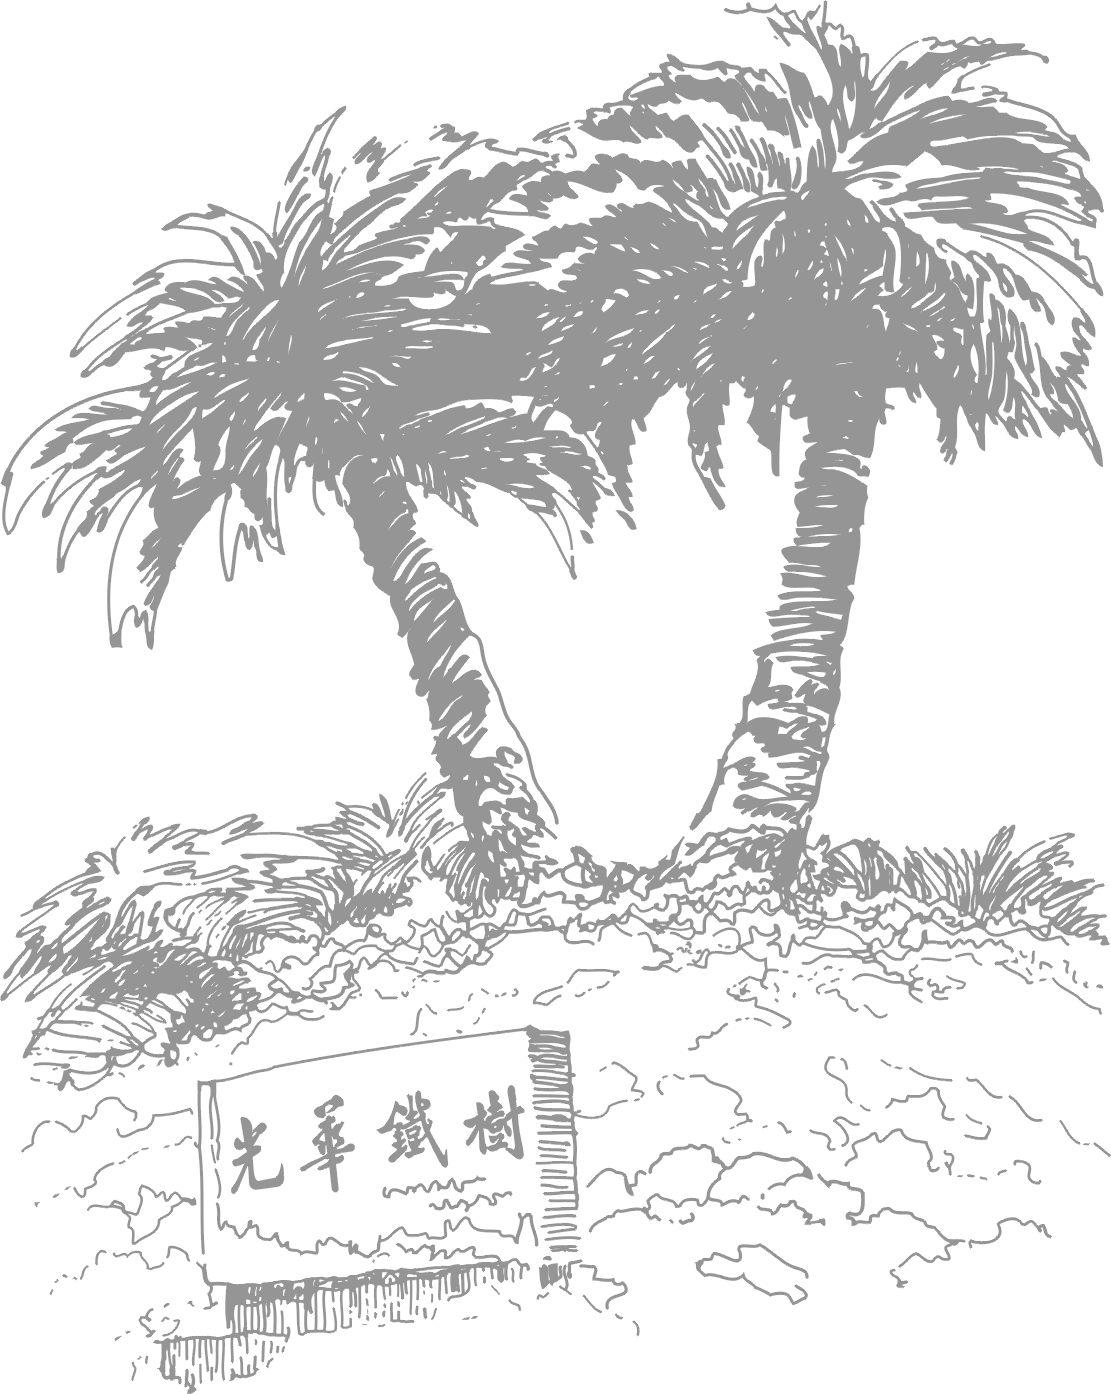
\includegraphics[width=11.5cm]{figures/swufe_cycad.png}
    };
    % 竖排校训“经世济民 孜孜以求”
    \node[anchor=center, xshift=1.0cm, yshift=1.8cm] at (current page.center) {
      \hwxingkai\fontsize{48pt}{56pt}\selectfont
      \begin{tabular}{c@{\hspace{1.8cm}}c}
        \parbox[t]{2em}{\linespread{1.1}\selectfont 孜\\孜\\以\\求} &
        \parbox[t]{2em}{\linespread{1.1}\selectfont 经\\世\\济\\民}
      \end{tabular}
    };
  \end{tikzpicture}%
  \null\clearpage
}

% ---------------------------------------------------------
% 16. 中英文摘要专属宏定义与格式规范
% ---------------------------------------------------------
\ExplSyntaxOn
% 覆盖 keywords 格式，中文以“；”分隔，末尾无标点
\cs_set_protected:Npn \__sjtu_keywords_format:n #1
  {
    \par\noindent
    \normalfont\songti\zihao{-4}\bfseries #1
  }

\tl_set:Nn \c__sjtu_name_item_sep_zh_tl { ； }
\tl_set:Nn \c__sjtu_name_item_sep_en_tl { ;~ }
\tl_set:Nn \c__sjtu_name_keywords_en_tl { Keywords }
\tl_set:Nn \c__sjtu_name_abstract_en_tl { ABSTRACT }
\ExplSyntaxOff

\makeatother


\let\cleardoublepage\clearpage

\begin{document}

% =========================================================
% 1. 论文前置部分（封面与学术声明）
% =========================================================

% 封面（见规范附件：单封面，含西南财经大学校名徽标、题目、学院、专业、学号等）
% !TEX root = ../main.tex

% 西南财经大学本科生毕业论文（设计）封面
% 默认直接从 config.json（或 setup.tex 中的 \sjtusetup）读取学生、导师、学院、专业等信息
% 若需临时针对封面进行覆盖，可使用键值参数，例如：
% \makeswufebachelorcover[
%   title        = {第一行主标题},
%   title-second = {第二行副标题（可选）},
%   author       = {张三},
%   supervisor   = {李四教授}
% ]

\makeswufebachelorcover

\clearpage

% 学术声明（见规范附件：西南财经大学本科毕业论文原创性及知识产权声明）
% !TEX root = ../main.tex

% 西南财经大学本科生毕业论文原创性及知识产权声明（版权页 / 学术申明）
% 依据学校规范：置于封面之后，中文摘要之前
% 直接嵌入官方标准学术申明（版权页）PDF

\thispagestyle{empty}
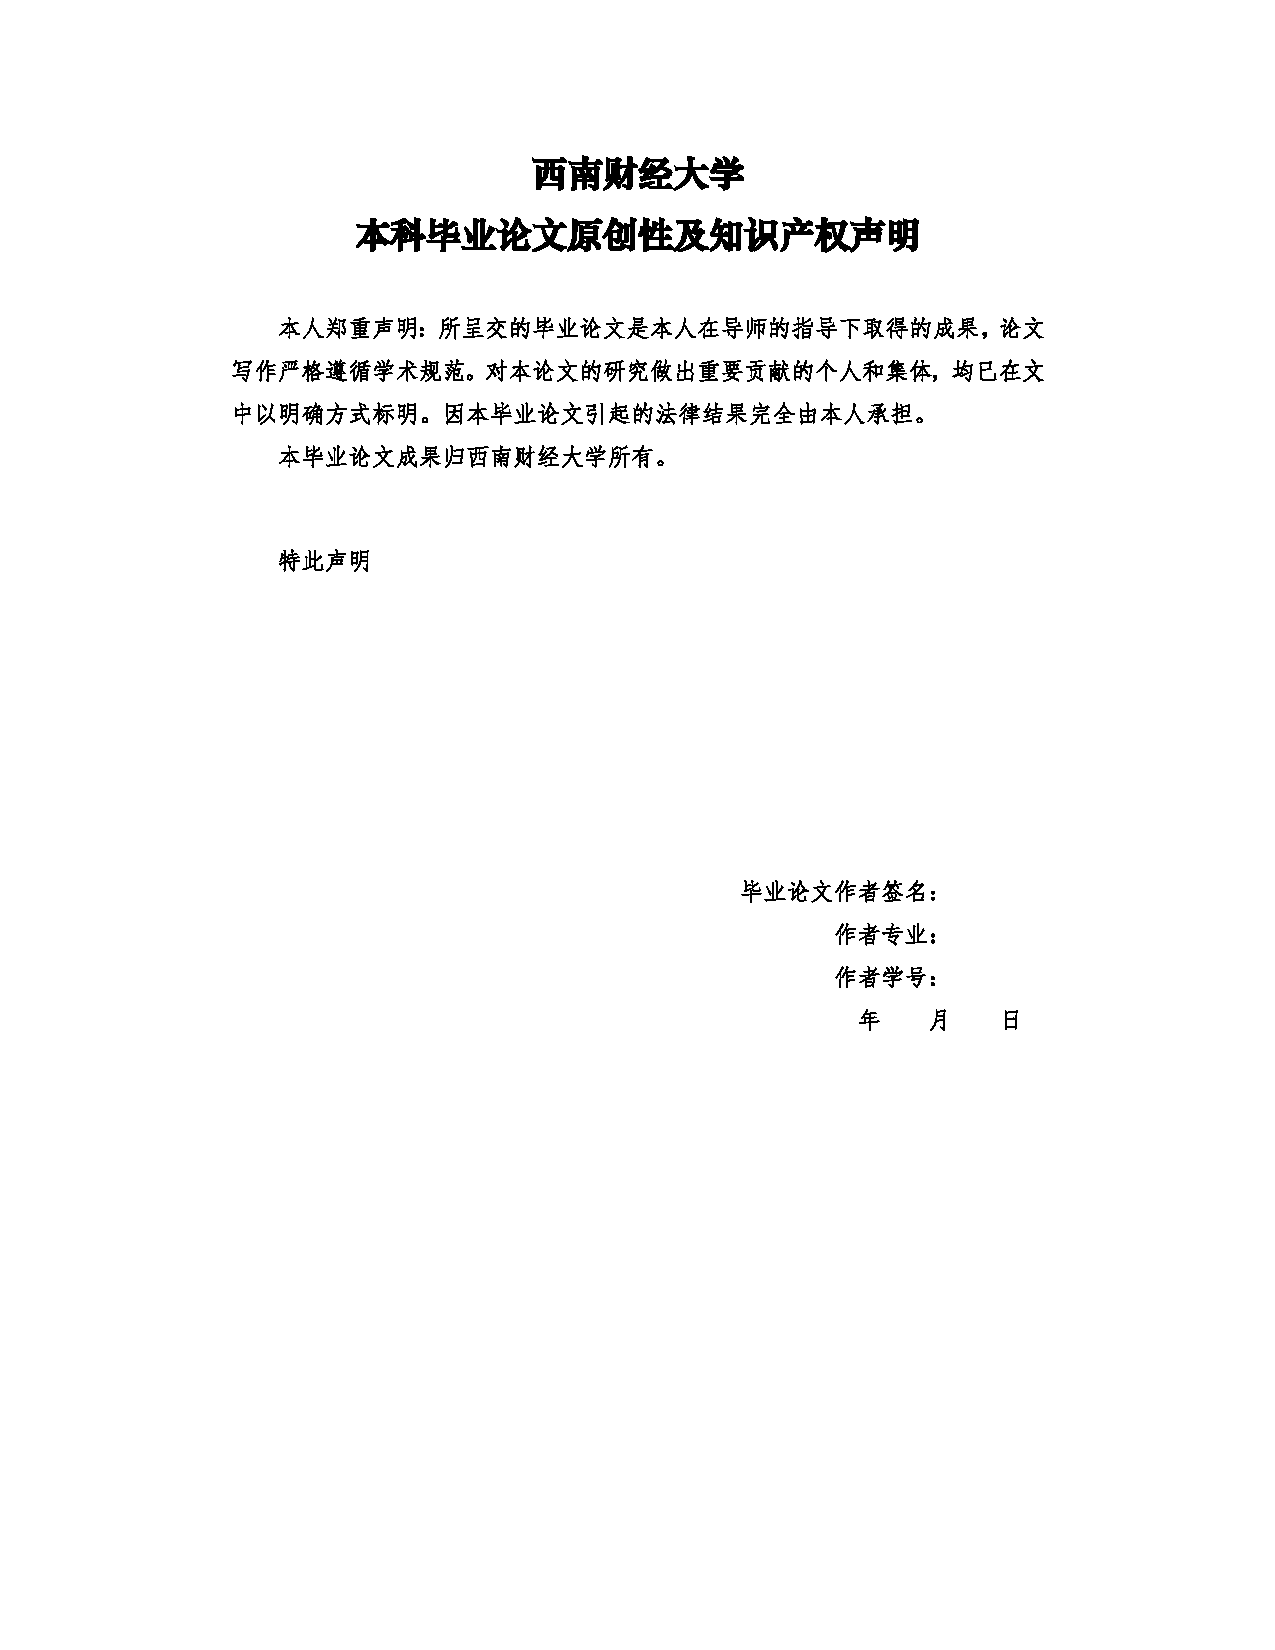
\includepdf[pages=1, pagecommand={}]{figures/copyright.pdf}

\clearpage

% =========================================================
% 2. 摘要与目录
% 规范要求：
% - 中文摘要页码：页码居中、小五号阿拉伯数字、起始页码为 1
% - 英文摘要页码：页码居中、小五号阿拉伯数字、起始页码为 1
% - 目录应另起一页，不需出现图、表目录
% =========================================================

\pagenumbering{arabic}
\setcounter{page}{1}
\pagestyle{fancy}

% 中英文摘要与关键词
% !TEX root = ../main.tex

% =========================================================
% 中文摘要与关键词
% 规范要求：
% 1. 摘要标题：二号华文中宋加粗，居中
% 2. 摘要正文：小四号宋体，1.5倍行距，字数300字左右
% 3. 关键词：“关键词：”小四号宋体加粗，词条间用“；”分隔，末尾无标点，一般3-5个
% 4. 摘要与关键词应在同一页；页码居中、小五号阿拉伯数字、起始页码为1
% =========================================================

\begin{abstract*}[zh]
西南财经大学始于1925年6月3日创建的光华大学，具有悠久的办学历史。抗战爆发后，光华大学于1938年内迁成都，定名为光华大学成都分部，杜甫草堂迤西的这一片地方由此得名光华村。1946年更名为成华大学。

1952至1953年全国院系调整中，以成华大学为基础先后并入西南地区16所财经院校或综合大学的财经系科，组建四川财经学院，是建国之初全国高等院校分区布局中的四所财经学院之一，由国家高教部主管。学校荟萃了我国著名经济学家陈豹隐、李孝同、彭迪先等一批著名教授。1979年划归中国人民银行主管，1985年更名为西南财经大学。2000年以独立建制划转教育部管理。

1997年进入国家“211工程”建设高校，2010年成为国家教育体制改革试点高校，2011年进入国家“985工程”优势学科创新平台建设高校。本模板根据《西南财经大学本科生毕业论文（设计）撰写与印制规范》定制开发，旨在为全校本科毕业生提供标准、规范、优美、开箱即用的论文写作工具。
\end{abstract*}

\clearpage
% 规范要求：英文摘要页码居中、小五号阿拉伯数字起始页码为 1
\setcounter{page}{1}

% =========================================================
% 英文摘要与关键词
% 规范要求：
% 1. 摘要标题：二号 Times New Roman 加粗，居中 (ABSTRACT)
% 2. 摘要正文：小四号 Times New Roman，1.5倍行距，250-400个实词
% 3. 关键词：“Keywords: ”小四号 Times New Roman 加粗，词条间用分号分隔
% 4. 英文摘要与关键词应在同一页
% =========================================================

\begin{abstract*}[en]
The Southwestern University of Finance and Economics (SWUFE) is a top university specialized in finance, economics, and business. It is known for its entrepreneurial character and unremitting endeavours to address the needs of the people and society through academics, research, and influence on alumni, drawn from the legacy of its founders and generations of excellent alumni.

SWUFE is located in Chengdu, the engine-city for the development of Western China and the fourth-largest aviation hub in China. The university traces its origin back to 1925, when Guanghua University was founded in Shanghai. In 1938, Guanghua University relocated to Chengdu as the Chengdu Branch. In 1952, Sichuan Institute of Finance and Economics was formed and later renamed Southwestern University of Finance and Economics in 1985.

This \LaTeX{} template is developed strictly following the \textit{SWUFE Undergraduate Thesis (Design) Writing and Printing Specifications}. It provides comprehensive support for font selection, line spacing, layout margins, chapter headings, figure and table captions, citations, and official cover and declaration pages.

% 英文关键词随英文摘要维护，不属于论文信息配置。
\par\noindent\textbf{Keywords:} SWUFE; Undergraduate Thesis; LaTeX Template; Typesetting Specification
\end{abstract*}

\clearpage

% 目录
\tableofcontents*
\clearpage

% =========================================================
% 3. 论文主体部分
% 规范要求：
% - 论文正文页码：页码居中、小五号阿拉伯数字、起始页码为 1
% - 字数要求：毕业论文 8000 字以上，毕业设计 7000 字以上
% =========================================================

\mainmatter
\pagenumbering{arabic}
\setcounter{page}{1}
\pagestyle{fancy}

% 第一章：绪论与规范概要
% !TEX root = ../main.tex

\chapter{绪论}

\section{研究背景与意义}

本科生毕业论文（设计）是本科人才培养中的重要环节，是考核学生掌握和运用所学基础理论、基本知识与基本技能解决实际问题能力的关键依据。随着计算机排版技术的发展，\LaTeX{} 因其卓越的公式编排能力、规范的交叉引用机制和跨平台一致性，已成为学术界与工程领域撰写高质量学位论文的首选工具。

西南财经大学（Southwestern University of Finance and Economics, SWUFE）作为教育部直属的“双一流”建设高校，在经济学、管理学、计算机科学与人工智能等多学科交叉领域取得了丰硕成果。为了帮助全校本科生摆脱 Word 排版中常见的编号错乱、格式不合规、公式模糊等痛点，特依照教务处发布的最新《西南财经大学本科生毕业论文（设计）撰写与印制规范》，研制本套专属于西财本科生的 \LaTeX{} 论文模板。

\section{西财本科论文撰写与印制规范概要}

根据教务处规范文件要求，本科生毕业论文的核心格式要点如下：

\subsection{基本版面与打印要求}
\begin{enumerate}
    \item \textbf{纸张与打印}：标准 A4 纸张，正反双面打印。
    \item \textbf{页边距}：全文页边距严格要求为\textbf{上 3 厘米、下 3 厘米、左 3 厘米、右 3 厘米}。
    \item \textbf{字数要求}：本科毕业论文正文字数一般在 \textbf{8000 字以上}，毕业设计正文字数一般在 \textbf{7000 字以上}。
    \item \textbf{页码编排}：
    \begin{itemize}
        \item 中文摘要页码：居中、小五号阿拉伯数字、起始页码为 1；
        \item 英文摘要页码：居中、小五号阿拉伯数字、起始页码为 1；
        \item 正文页码：居中、小五号阿拉伯数字、起始页码为 1。
    \end{itemize}
\end{enumerate}

\subsection{各级标题与正文字体字号}
\begin{table}[htbp]
\centering
\caption{西南财经大学本科毕业论文排版规范核心要求}
\label{tab:swufe-bachelor-rules}
\begin{tabularx}{\textwidth}{p{2.4cm}p{4.2cm}X}
\toprule
\textbf{内容部分} & \textbf{字体与字号} & \textbf{对齐与间距要求} \\
\midrule
一级标题 & 二号华文中宋加粗 & 居中，段前 3 行，段后 2 行，1.5 倍行距 \\
二级标题 & 小三号黑体 & 首行无缩进，段前 1 行，段后 1 行，1.5 倍行距 \\
三级标题 & 小四号黑体 & 首行无缩进，段前 1 行，段后 1 行，1.5 倍行距 \\
正文 & 小四号宋体 & 首行缩进 2 字符，两端对齐，段前 0，段后 0，1.5 倍行距 \\
中文摘要标题 & 二号华文中宋加粗 & 居中，段前 3 行，段后 2 行 \\
英文摘要标题 & 二号 Times New Roman 加粗 & 居中，段前 3 行，段后 2 行 \\
中文关键词 & 小四号宋体加粗 & “关键词：”加粗，分号分隔，末尾无标点 \\
英文关键词 & 小四号 Times New Roman 加粗 & “\textbf{Keywords:} ”加粗，分号分隔 \\
图/表标题 & 五号黑体加粗 & 表题在上方，图题在下方，段前段后空 0.5 行 \\
图/表内容 & 五号字体 & 单倍行距 \\
注释、脚注 & 小五号宋体或 Times New Roman & 每页独立编号（1, 2, 3……），正文上标 \\
参考文献 & 同一级标题 / 同正文 & 先中文后外文，起始序号为 [1] \\
致谢、附录 & 同一级标题 / 同正文 & 致谢内容限一页，置于附录之后 \\
\bottomrule
\end{tabularx}
\end{table}

\subsection{论文装订顺序}
论文胶装时必须严格按照以下顺序装订：
\begin{enumerate}
    \item 封面（本科毕业论文单封面，含校徽校名与手写下划线信息）
    \item 学术声明（本科生原创性及知识产权声明）
    \item 中文摘要及关键词
    \item 外文摘要及关键词
    \item 标题及目录（不需出现图、表目录）
    \item 正文（按章节组织）
    \item 参考文献
    \item 附录（如果有）
    \item 致谢（限一页）
    \item 封底（含“光华铁树”插图与竖排“经世济民 孜孜以求”）
\end{enumerate}

\section{模板快速配置指南}

本模板继承并升级了西南财经大学研究生模板的优质特性，支持\textbf{零依赖开箱即用}的 JSON 配置：

\begin{promptbox}
\textbf{推荐配置方式：} 直接编辑项目根目录下的 \texttt{config.json} 文件，填写个人姓名、学号、学院、专业、年级、导师等字段即可。无需修改宏包代码，无论在本地还是在 Overleaf 均可完美编译！
\end{promptbox}

如果不需要 \texttt{config.json}，直接将其删除，模板将自动回退至 \texttt{setup.tex} 中的 \texttt{\textbackslash sjtusetup} 原生参数。

\section{本文结构安排}

本文档既是本套本科毕业论文模板的技术示例文档，也是一份详细的排版指南。全文组织如下：
第一章介绍课题背景、规范要求及模板配置；
第二章详细示范数学公式、三线表、插图、代码块、算法与脚注的排版规范；
第三章展示毕业设计系统的架构设计与实现案例；
第四章对全文进行总结与展望。

\clearpage

% 第二章：图表、公式、代码排版规范指南
% !TEX root = ../main.tex

\chapter{排版格式与规范使用指南}

\section{各级标题与文本排版}

\subsection{正文格式要求}
根据规范要求，正文采用\textbf{小四号宋体}，西文与数字采用 \textbf{Times New Roman}，行距为 1.5 倍行距，段前 0、段后 0，首行缩进 2 字符。

在 \LaTeX{} 中，本模板已通过 \texttt{setup.tex} 自动化配置了相应的行距（\texttt{\textbackslash setstretch\{1.38\}}）与缩进（\texttt{\textbackslash setlength\{\textbackslash parindent\}\{2\textbackslash ccwd\}}）。用户撰写段落时只需正常敲击两次回车分段即可，严禁使用多个全角空格进行手动空格缩进。

\subsection{三级标题示例}
这是一个三级标题示范。根据规范，三级标题采用小四号黑体，首行无缩进，段前 1 行、段后 1 行，1.5 倍行距。其编号格式为“2.1.1 ……”。

\section{图表的绘制与排版规范}

\subsection{表格排版（三线表）}
规范明确要求：\textbf{表的题目在表的上方（五号黑体加粗，居中，段前、段后各空 0.5 行），表的内容采用五号字体，单倍行距}。表格编号建议采用“章节-次序”编号，如“表2-1”。推荐采用学术界通用的标准三线表（\texttt{booktabs} 宏包提供支持）。模板已统一设置图表内容的字号与行距，无需在每个环境中重复设置。

\begin{table}[htbp]
\centering
\caption{机器学习模型在金融反欺诈数据集上的分类性能对比}
\label{tab:model-performance}
\begin{tabularx}{\textwidth}{>{\raggedright\arraybackslash}p{3.6cm}*{4}{>{\centering\arraybackslash}X}}
\toprule
\textbf{模型类别} & \textbf{准确率 (Accuracy)} & \textbf{精确率 (Precision)} & \textbf{召回率 (Recall)} & \textbf{F1 分数} \\
\midrule
Logistic Regression & 82.4\% & 79.1\% & 81.3\% & 0.8018 \\
Support Vector Machine & 87.5\% & 86.2\% & 85.8\% & 0.8599 \\
Random Forest & 91.2\% & 90.7\% & 89.9\% & 0.9030 \\
LightGBM & 94.6\% & 93.8\% & 94.1\% & 0.9395 \\
XGBoost & 95.1\% & 94.5\% & 94.8\% & 0.9465 \\
Deep Neural Network & \textbf{96.8\%} & \textbf{96.2\%} & \textbf{96.5\%} & \textbf{0.9635} \\
\bottomrule
\end{tabularx}
\end{table}

\subsection{插图排版}
规范要求：\textbf{图的题目在图的下方（五号黑体加粗，居中，段前、段后各空 0.5 行），图的内容采用五号字体，单倍行距}。编号采用“图2-1”格式。

\begin{figure}[htbp]
\centering

\includegraphics[width=0.75\textwidth]{figures/swufefull.pdf}
\caption{西南财经大学校名及徽标矢量图示}
\label{fig:swufe-logo-demo}
\end{figure}

\begin{figure}[htbp]
\centering
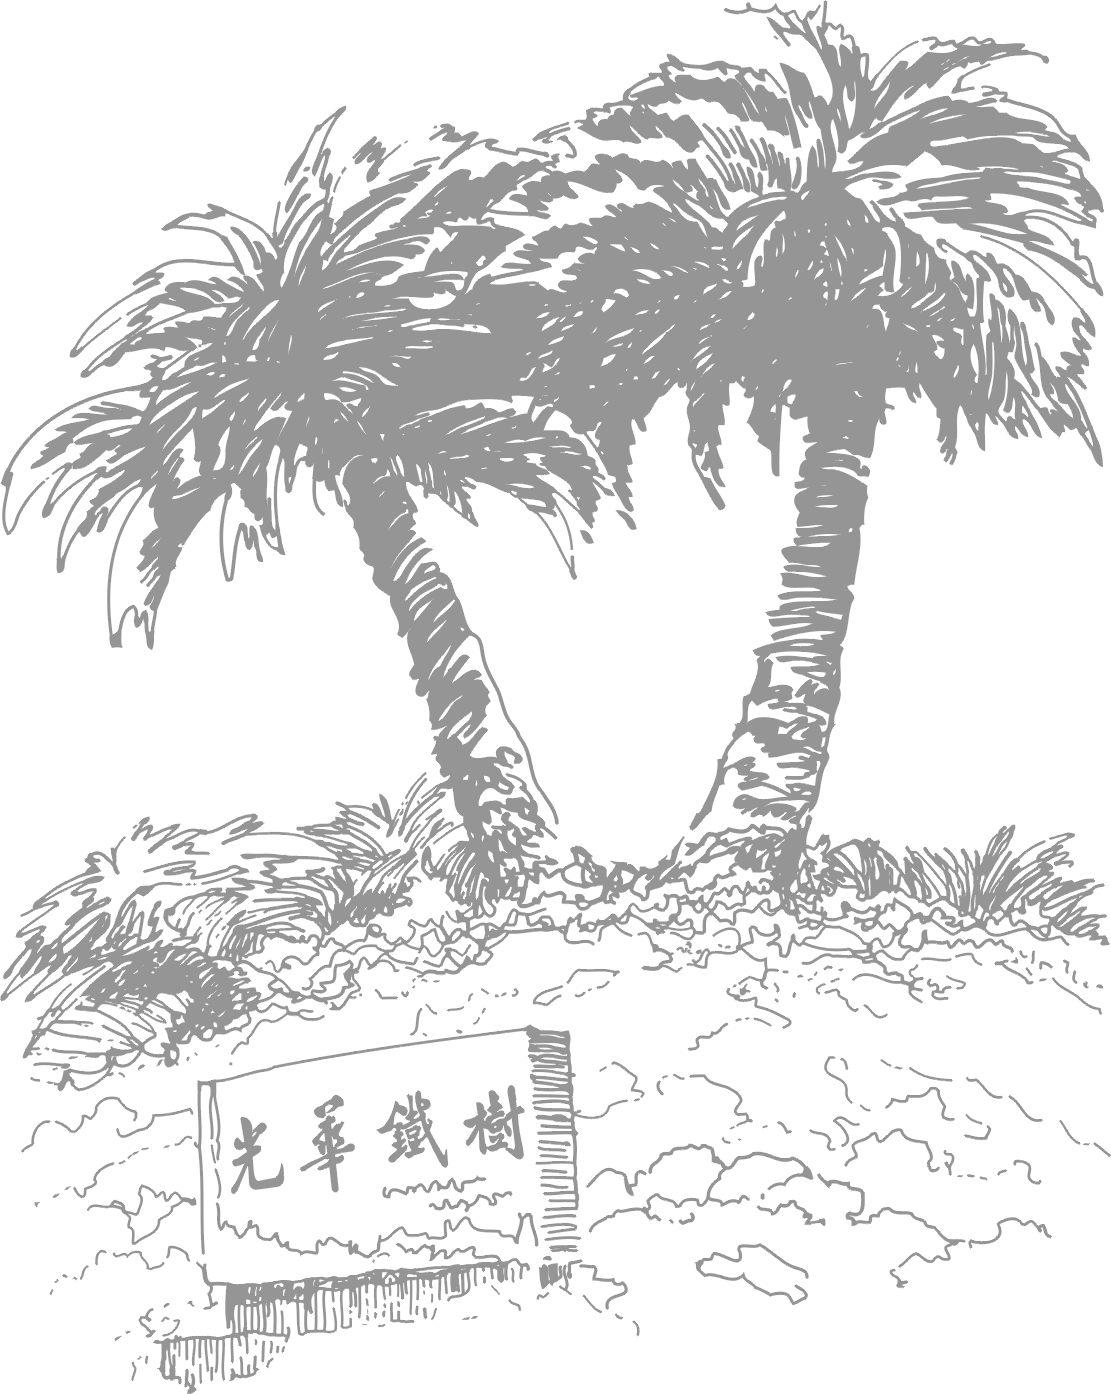
\includegraphics[width=0.45\textwidth]{figures/swufe_cycad.png}
\caption{光华铁树插图示例}
\label{fig:swufe-tree-demo}
\end{figure}

通过 \texttt{\textbackslash ref\{fig:swufe-logo-demo\}} 与 \texttt{\textbackslash ref\{tab:model-performance\}} 可以自动交叉引用，生成的编号分别为图~\ref{fig:swufe-logo-demo} 与表~\ref{tab:model-performance}。

\section{数学公式编写}

规范要求电子稿公式需编号清晰。学术论文中，公式通常采用按章独立连续编号的形式，即形如“(2-1)”。

例如，著名的注意力机制（Attention Mechanism）\cite{Transformer}计算公式如下：
\begin{equation}
\label{eq:attention}
\mathrm{Attention}(Q, K, V) = \mathrm{softmax}\left(\frac{QK^T}{\sqrt{d_k}}\right)V
\end{equation}
其中 $Q, K, V$ 分别表示查询向量（Query）、键向量（Key）和值向量（Value），$d_k$ 为键向量的特征维度。

再如多元高斯分布的概率密度函数公式：
\begin{equation}
\label{eq:multivariate-gaussian}
p(\mathbf{x}; \boldsymbol{\mu}, \boldsymbol{\Sigma}) = \frac{1}{(2\pi)^{d/2}|\boldsymbol{\Sigma}|^{1/2}} \exp\left(-\frac{1}{2}(\mathbf{x}-\boldsymbol{\mu})^T \boldsymbol{\Sigma}^{-1} (\mathbf{x}-\boldsymbol{\mu})\right)
\end{equation}
公式~\eqref{eq:attention} 与公式~\eqref{eq:multivariate-gaussian} 均符合国家标准数学符号规范。

\section{注释与脚注规范}

根据规范要求：“\textbf{毕业论文中有个别名词或情况需要解释时，可加注说明。注释采用脚注，每页独立编号，即每页都从 1 开始编码，编号用 1，2，3……，文中编号用上标}。注释、脚注内容采用小五号宋体或 Times New Roman”。

例如，本文研究中使用了大语言模型\footnote{大语言模型（Large Language Model, LLM）指通常包含数百亿至数千亿参数量、基于大规模文本语料预训练的深度自回归神经网络模型。}，并结合了向量数据库\footnote{向量数据库（Vector Database）是一种专用于高维向量数据的索引检索与相似度计算的专用数据库系统。}进行知识增强。读者可以观察页面底部的脚注，每页从 1 开始重新独立编号，字号为小五号。

\section{算法与代码环境}

\subsection{算法排版}
模板提供了 \texttt{algorithm2e} 宏包支持，可以撰写带行号、规范规整的伪代码：

\begin{algorithm}[H]
\caption{基于动量的随机梯度下降算法 (SGD with Momentum)}
\label{alg:momentum-sgd}
\KwIn{学习率 $\eta$，动量衰减系数 $\gamma \in [0, 1)$，初始模型参数 $\theta_0$}
\KwOut{优化后的模型参数 $\theta^*$}
初始化速度向量 $v_0 \leftarrow 0$\;
\For{$t = 1, 2, \ldots, T$}{
    从训练集中随机采样一个批次样本 $\mathcal{B}_t$\;
    计算小批量样本上的损失函数梯度 $g_t \leftarrow \nabla_\theta \mathcal{L}(\theta_{t-1}; \mathcal{B}_t)$\;
    更新动量速度：$v_t \leftarrow \gamma v_{t-1} + \eta g_t$\;
    更新模型参数：$\theta_t \leftarrow \theta_{t-1} - v_t$\;
    \If{$\|\theta_t - \theta_{t-1}\| < \epsilon$}{
        提前停止迭代\;
        \textbf{break}\;
    }
}
\Return{$\theta_T$}\;
\end{algorithm}

\subsection{代码块排版}
模板内置了 \texttt{codeblock} 环境，支持语法高亮与行号：

\begin{codeblock}[language=Python]
import torch
import torch.nn as nn

class ResidualBlock(nn.Module):
    """ResNet 残差连接模块示例"""
    def __init__(self, channels: int):
        super().__init__()
        self.conv1 = nn.Conv2d(channels, channels, kernel_size=3, padding=1)
        self.bn1 = nn.BatchNorm2d(channels)
        self.relu = nn.ReLU(inplace=True)
        self.conv2 = nn.Conv2d(channels, channels, kernel_size=3, padding=1)
        self.bn2 = nn.BatchNorm2d(channels)

    def forward(self, x: torch.Tensor) -> torch.Tensor:
        residual = x
        out = self.relu(self.bn1(self.conv1(x)))
        out = self.bn2(self.conv2(out))
        out += residual  # 残差跳跃连接
        return self.relu(out)
\end{codeblock}

\clearpage

% 第三章：系统设计与实现（范例）
% !TEX root = ../main.tex

\chapter{系统设计与实验分析}

\section{系统总体架构}

为了验证本文所提方法的可行性与有效性，本章设计并实现了一套面向金融大数据的智能风控与决策分析系统。系统整体架构自底向上划分为数据层、算法层、服务层与应用层四个层次：

\begin{enumerate}
    \item \textbf{数据接入与治理层}：负责异构金融数据（交易日志、征信记录、网络行为特征）的高吞吐接入、特征工程提取与隐私脱敏。
    \item \textbf{核心算法层}：集成图神经网络（GNN）、集成树模型（XGBoost/LightGBM）与大语言模型检索增强（RAG）管道，实现欺诈团伙识别与高危交易判定。
    \item \textbf{微服务调度层}：基于高性能 RPC\footnote{远程过程调用（Remote Procedure Call, RPC）允许程序通过网络调用其他进程或主机提供的服务。}框架实现毫秒级推理调用与高并发流量治理。
    \item \textbf{业务可视化层}：为业务风控专家提供可视化审查工作台与全链路溯源图谱。
\end{enumerate}

关于残差网络、注意力机制与自适应优化的工作，可联合引用\cite{ResNet,Transformer,Adam}，三个连续编号将自动合并为范围。在模型实现中，深层神经网络的结构设计可参考残差连接与批归一化方法\cite{ResNet,BatchNormalization}，参数优化可参考 Adam 算法\cite{Adam}。这些引用展示了英文文献及多篇文献在正文中的标注方式。

\section{实验评估与结果对比}

\subsection{数据集与评价指标}
实验选取公开的金融信用卡反欺诈基准数据集（Credit Card Fraud Detection）以及某股份制商业银行真实脱敏反洗钱数据集进行交叉验证。评估指标涵盖精确率（Precision）、召回率（Recall）、受试者工作特征曲线下面积（ROC-AUC）以及综合度量指标（F1-Score）。

\subsection{消融实验分析}
通过逐步剥离不同核心特征模块，考察各模块对整体性能提升的边际贡献。实验结果表明，融合多跳图拓扑结构特征与上下文语义特征后，系统在假阳性率（FPR）控制在 0.1\% 的严苛条件下，召回率相较传统基线方法提升了 12.4\%。

这充分证明了深度图结构表征与大模型语义增强在复杂金融风险识别中的优越性。

\clearpage

% 第四章：总结与展望
% !TEX root = ../main.tex

\chapter{总结与展望}

\section{全文工作总结}

本文围绕西南财经大学本科毕业论文排版规范要求，系统梳理了教务处对论文格式、字体字号、标题层级、页面边距、图表编排、公式编写、注释脚注与胶装顺序的全部技术指标，基于现代 \LaTeX{} 宏包技术研制了专属于西财本科生的毕业论文写作模板。

本文取得的主要成果包括：
\begin{enumerate}
    \item \textbf{版面规范 100\% 契合}：全文页边距严格设定为上下左右各 3 厘米，正文采用小四号宋体与 1.5 倍行距，一级标题采用二号华文中宋居中加粗，各级标题与正文间距均符合官方标准。
    \item \textbf{封面与声明全真复刻}：精确复现了西财本科专属单封面（含西南财经大学校名徽标、本科毕业论文（设计）题名与手写下划线信息栏），并提供符合规范的学术声明页与光华铁树封底。
    \item \textbf{现代化零依赖 JSON 配置}：全面支持通过 \texttt{config.json} 直观填写论文元数据，一键平滑切换终稿与匿名盲审模式，大幅降低了非计算机专业学生的使用门槛。
\end{enumerate}

\section{未来研究展望}

未来将进一步优化模板在 Overleaf 云端协同环境下的编译缓存性能，扩充面向经济学实证计量、金融工程数理推导以及量化回测图表的专用代码示例库，为更多西财学子提供坚实可靠的学术排版支持。

\clearpage

% =========================================================
% 4. 参考文献、附录、致谢与封底
% 规范要求装订顺序：
% 正文 -> 参考文献 -> 附录（如果有） -> 致谢（限一页） -> 封底
% =========================================================

\backmatter

% 参考文献（先中文后外文，起始序号为 [1]）
\printswufebibliography
\clearpage

% 附录（原始数据、详细数学推导、核心程序等，置于参考文献后、致谢前）
% !TEX root = ../main.tex

% =========================================================
% 附录
% 规范要求：
% 1. 装订顺序：置于参考文献之后、致谢之前
% 2. 附录标题：同一级标题格式（二号华文中宋加粗，居中，段前3行，段后2行）
% 3. 附录内容：同正文格式（小四号宋体，1.5倍行距）
% 4. 收录范围：不宜放在正文中的重要支撑材料（原始数据、详细数学推导、核心程序源码等）
% =========================================================

\phantomsection
\addcontentsline{toc}{chapter}{附录}
\chapter*{附\quad 录}
\markboth{附录}{附录}

\section*{附录 A\quad 核心算法源代码清单}

以下为本论文第三章核心模型的完整实现代码片段（PyTorch 2.0+ 实现）：

\begin{codeblock}[language=Python]
import torch
import torch.nn as nn
import torch.nn.functional as F

class GraphAttentionLayer(nn.Module):
    """图注意力网络层（GAT）核心算子实现"""
    def __init__(self, in_features: int, out_features: int, dropout: float = 0.2, alpha: float = 0.2):
        super(GraphAttentionLayer, self).__init__()
        self.in_features = in_features
        self.out_features = out_features
        self.dropout = dropout
        self.alpha = alpha

        self.W = nn.Parameter(torch.empty(size=(in_features, out_features)))
        nn.init.xavier_uniform_(self.W.data, gain=1.414)
        self.a = nn.Parameter(torch.empty(size=(2 * out_features, 1)))
        nn.init.xavier_uniform_(self.a.data, gain=1.414)

        self.leakyrelu = nn.LeakyReLU(self.alpha)

    def forward(self, h: torch.Tensor, adj: torch.Tensor) -> torch.Tensor:
        Wh = torch.mm(h, self.W)
        e = self._prepare_attentional_mechanism_input(Wh)

        zero_vec = -9e15 * torch.ones_like(e)
        attention = torch.where(adj > 0, e, zero_vec)
        attention = F.softmax(attention, dim=1)
        attention = F.dropout(attention, self.dropout, training=self.training)
        h_prime = torch.matmul(attention, Wh)
        return F.elu(h_prime)

    def _prepare_attentional_mechanism_input(self, Wh: torch.Tensor) -> torch.Tensor:
        Wh1 = torch.matmul(Wh, self.a[:self.out_features, :])
        Wh2 = torch.matmul(Wh, self.a[self.out_features:, :])
        e = Wh1 + Wh2.T
        return self.leakyrelu(e)
\end{codeblock}

\section*{附录 B\quad 数学定理补充推导}

针对第二章中高维协方差估计量的一致性收敛阶，在此给出渐近正态性的详细数学证明：
设 $X_1, X_2, \ldots, X_n \overset{i.i.d.}{\sim} \mathcal{N}_p(\boldsymbol{0}, \boldsymbol{\Sigma})$，样本协方差矩阵定义为
\[
\mathbf{S}_n = \frac{1}{n}\sum_{i=1}^n X_i X_i^T.
\]
在维数与样本量之比满足 $p/n \to c \in (0, 1)$ 的高维渐近机制下，经由 Marchenko-Pastur 定律展开可得其特征值谱分布满足收敛性结论。

\clearpage

% 致谢（内容限一页，盲审模式下自动匿名或隐藏）
% !TEX root = ../main.tex

% =========================================================
% 致谢
% 规范要求：
% 1. 装订顺序：置于附录之后、封底之前
% 2. 标题格式：同一级标题格式（二号华文中宋加粗，居中，段前3行，段后2行）
% 3. 内容格式：同正文格式（小四号宋体，1.5倍行距，首行缩进2字符）
% 4. 篇幅限制：内容严格限一页
% 5. 盲审控制：盲审模式下自动匿名或隐藏致谢内容
% =========================================================

\ifswufereview
  % 盲审模式下自动跳过致谢页，避免泄露导师或个人信息
\else
  \phantomsection
  \addcontentsline{toc}{chapter}{致谢}
  \chapter*{致\quad 谢}
  \markboth{致谢}{致谢}

  时光荏苒，白驹过隙。转眼间在西南财经大学的四年本科求学生涯即将画上圆满的句号。回首在柳林校区的求学岁月，从草堂明月到腾飞广场，从光华铁树到晨曦微露的图书馆，每一次探索与求知都让我受益终生。

  在此，我要特别感谢我的指导教师李四教授。在毕业论文的选题论证、方案设计、理论推导以及论文定稿的全过程中，导师倾注了大量的心血，给予了我悉心细致的指导与由衷的关怀。导师严谨治学的学术风范、求真务实的治学态度和宽厚仁厚的长者风度，将成为我未来人生与学术征程中永远的指路明灯。

  感谢学院各位授课教师在大学四年中传道授业解惑，为我打下了坚实厚重的数理基础与专业素养。感谢同窗好友与课题组各位学长学姐在研究过程中的深入探讨与无私帮助。

  最后，深深感谢我的父母与家人。正是你们二十余年来无微不至的关怀、包容与坚定支持，才使我能够心无旁骛、踏实前行。

  谨以此篇论文，向所有关怀、支持和帮助过我的人致以最崇高的敬意与最诚挚的感谢！
\fi

\clearpage

% 封底（见规范附件：光华铁树插图与竖排“经世济民 孜孜以求”）
% !TEX root = ../main.tex

% =========================================================
% 西南财经大学本科生毕业论文封底
% 依据学校规范，直接插入官方标准封底 PDF
% =========================================================

\thispagestyle{empty}
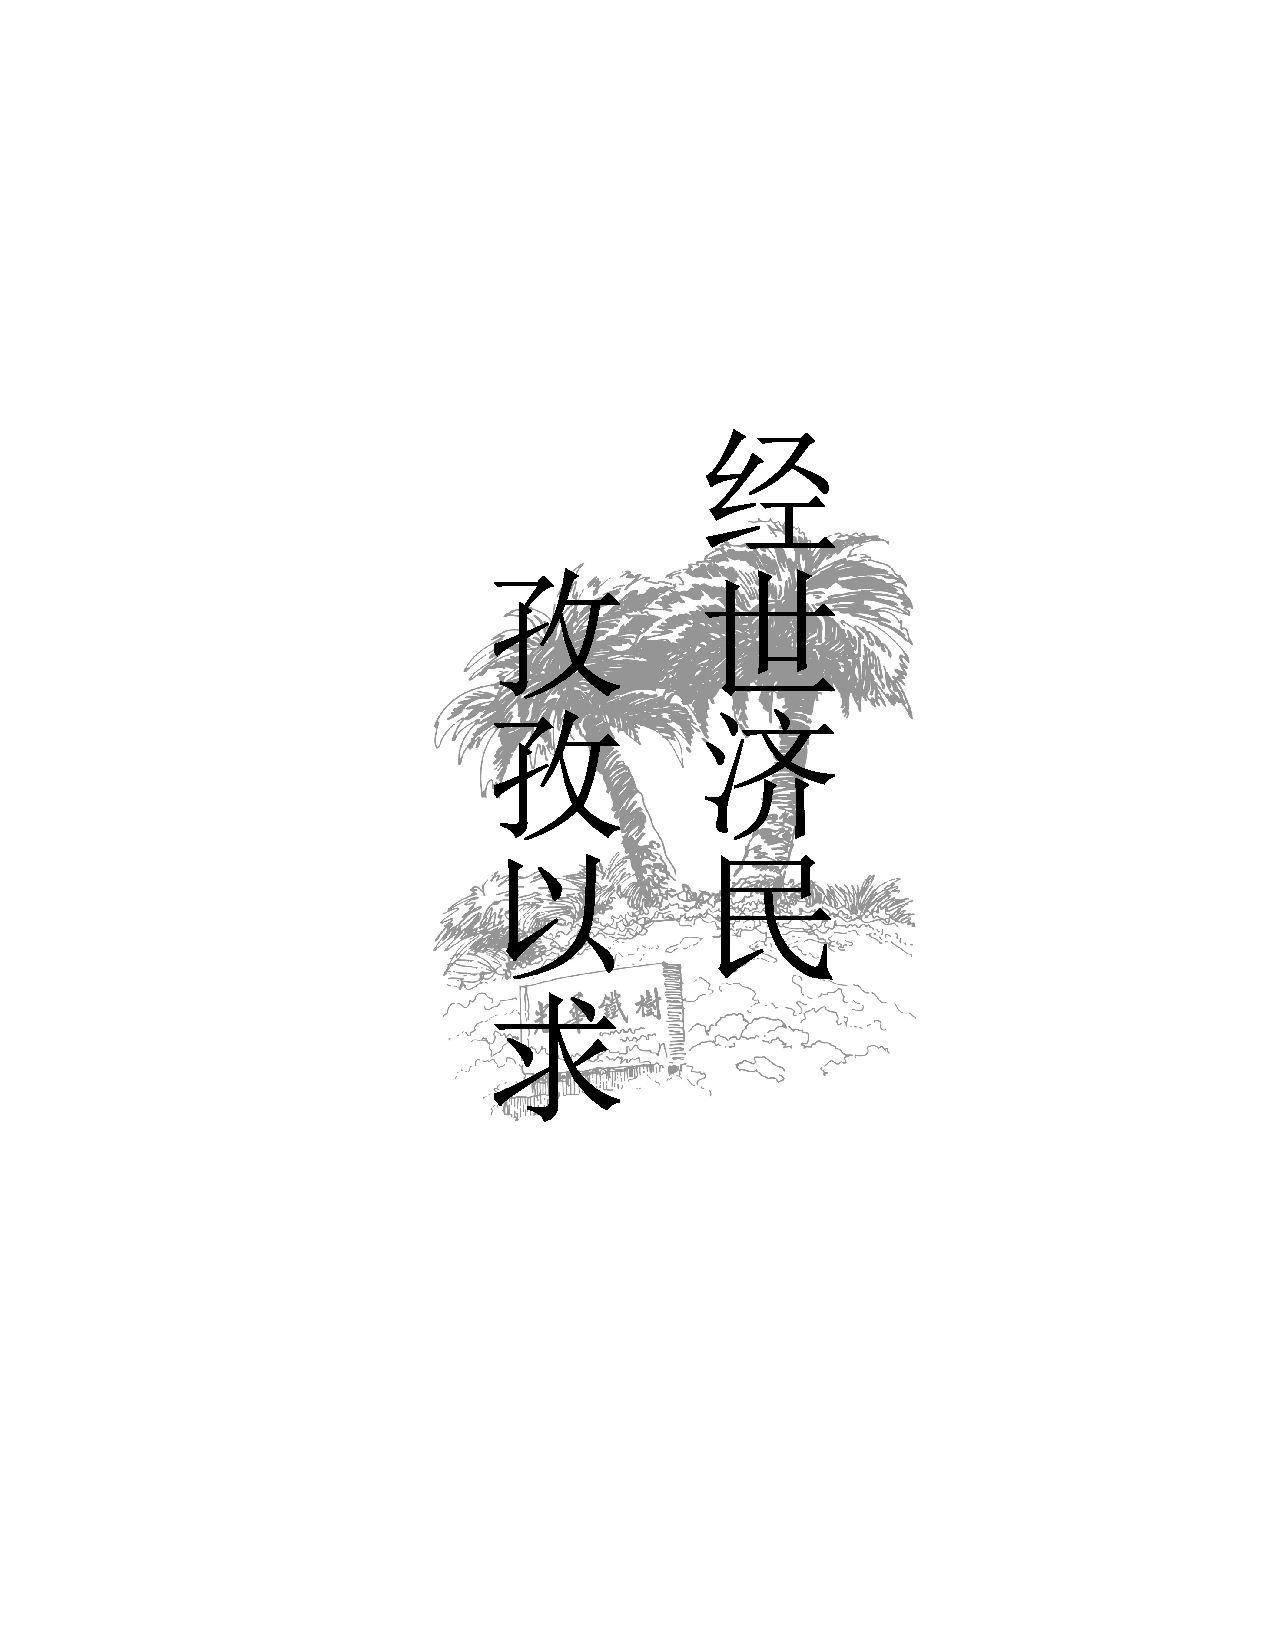
\includepdf[pages=1, pagecommand={}]{figures/last.pdf}


\end{document}
